\chapter{Data}
\label{chap:data}

This chapter discusses the datasets used in the thesis, as well as the pre and post-processing steps that are performed in order to facilitate the training and validation of the proposed method. In addition to this, a couple of concepts that motivate the choices or that are directly used in the process of the data are explained with the help of illustrations. 

The main dataset used in the thesis is \textit{Human3.6M}: Large Scale Datasets and Predictive Methods for 3D Human Sensing in Natural Environments \cite{H3.6}. Most of the related works benchmark their methods on Human3.6M and it also is freely accessible to academics on request. For further evaluation of model performance in the wild, outdoor datasets that do not have 3D ground truth such as \textit{3DPW}: 3D Poses in the Wild \cite{3dpw} would be used.

\begin{figure}[h]
    \centering
    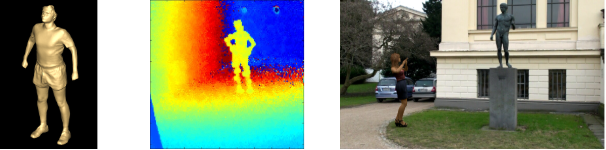
\includegraphics[width=\textwidth]{figures/h36/modlities.png}
    \caption{Additional modalities such as (from left to right) Full body model, depth from time of flight and mixed reality data are availble in Human3.6M dataset \cite{H3.6}. These datasets can be used for human body estimation, depth map estiamtion or inferring absolute 2D or 3D pose directly from full image i.e without cropping the region with a single person.}
    \label{fig:h36_modality}
\end{figure}

\section{Human3.6M}
\label{sec:h36m}
Human3.6M is a large scale indoor dataset with 3.6 million human poses collected with 4 cameras at different angles using a highly accurate maker-based \ac{mocap} system. The dataset constitutes 15 diverse motion and actions in various everyday scenarios namely, Directions, Discussion, Eating, Greeting, Phoning, Photo, Posing, Purchases, Sitting, Sitting Down, Smoking, Waiting, WalkDog, Walking, and WalkTogether. These actions are performed by 11 professional actors wearing a variety of realistic clothing. The datasets provides synchronized 2D and 3D data including full-body scans as shown in Fig \ref{fig:h36_modality}. It also includes mixed-reality test data created using animated human models to cover huge variations of background, clothing, illumination, occlusion, and camera angles.

The data of interest is mainly the 2D pose for training, 3D poses for evaluation and images for qualitative analysis as it is sometimes challenging even for the human eye to estimate 3D pose just from the 2D skeleton. Both the poses are composed of 17 joints or keypoint annotations namely, Pelvis (also referred to as Root), Torso, Neck, Nose, Head, right and left - Hip, Knee, Ankle, Shoulder, Elbow, Wrist. An image sample from the dataset with its corresponding 2D and 3D pose is illustrated in the Fig \ref{fig:h36_sample}. 

\begin{figure}
    \centering
    \begin{subfigure}[b]{0.3\textwidth}
        \centering
        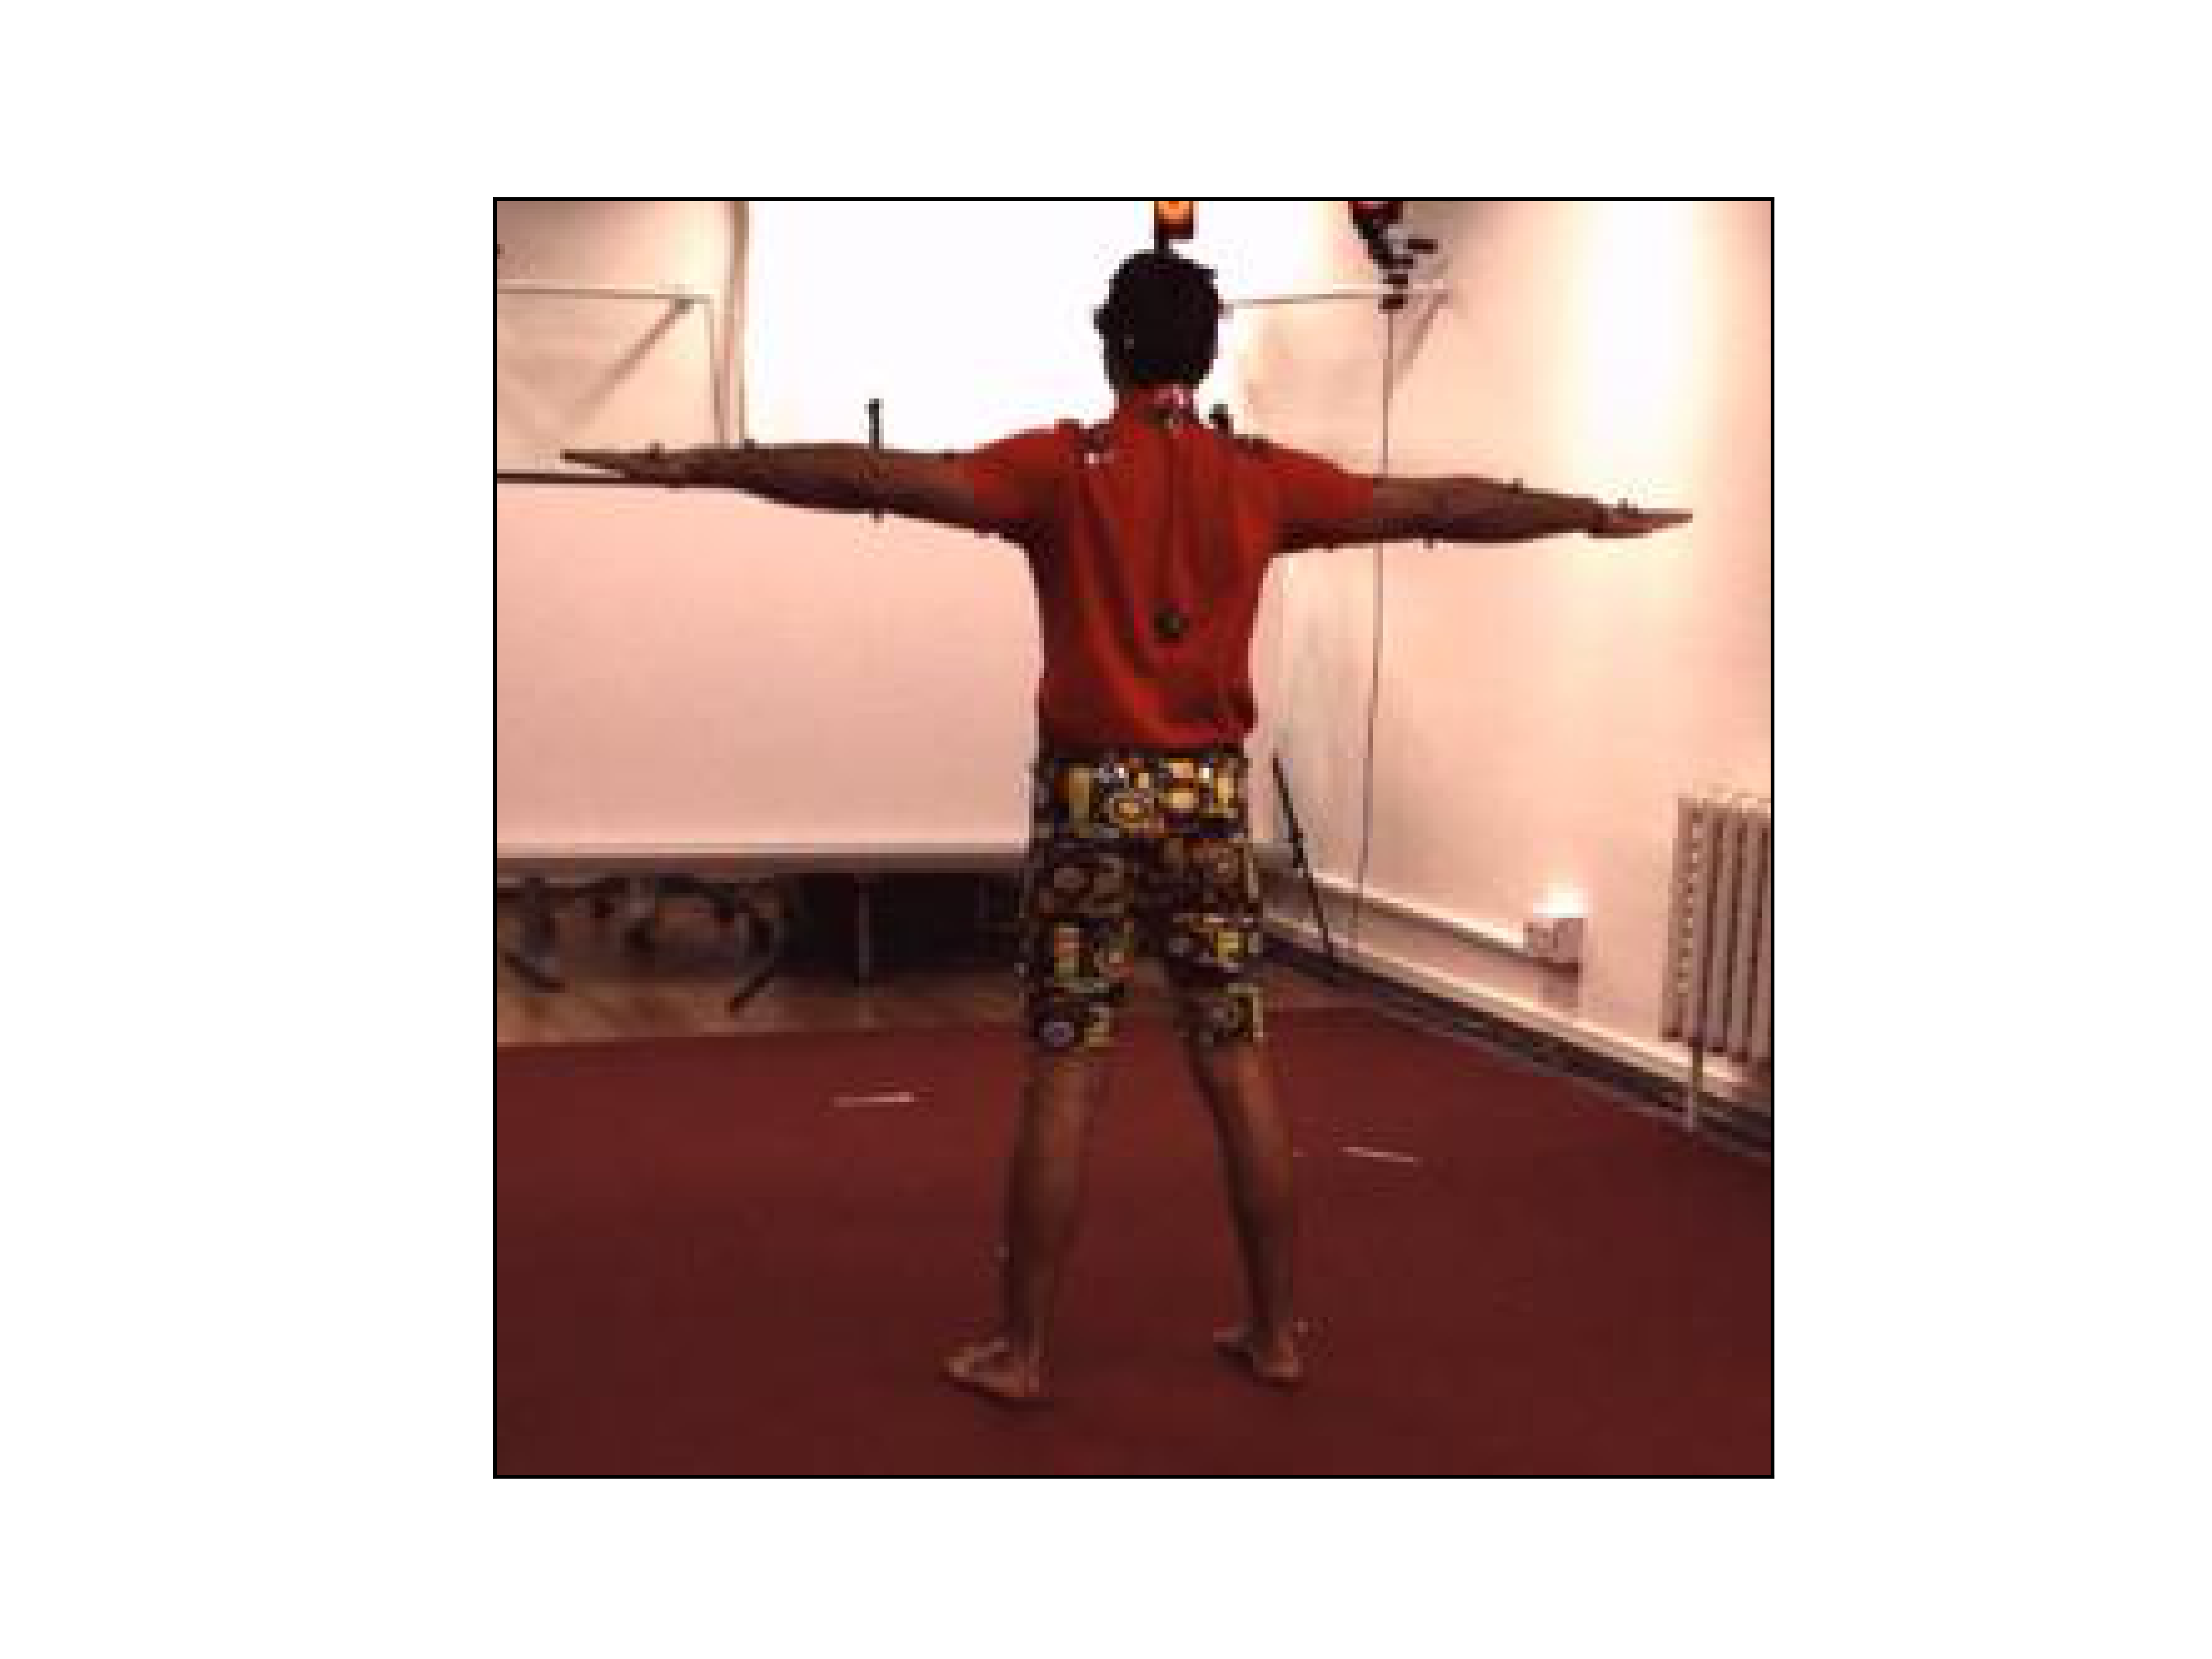
\includegraphics[width=\textwidth]{figures/h36_viz/h36image.png}
        \caption{}
    \end{subfigure}
    \hfill
    \begin{subfigure}[b]{0.3\textwidth}
        \centering
        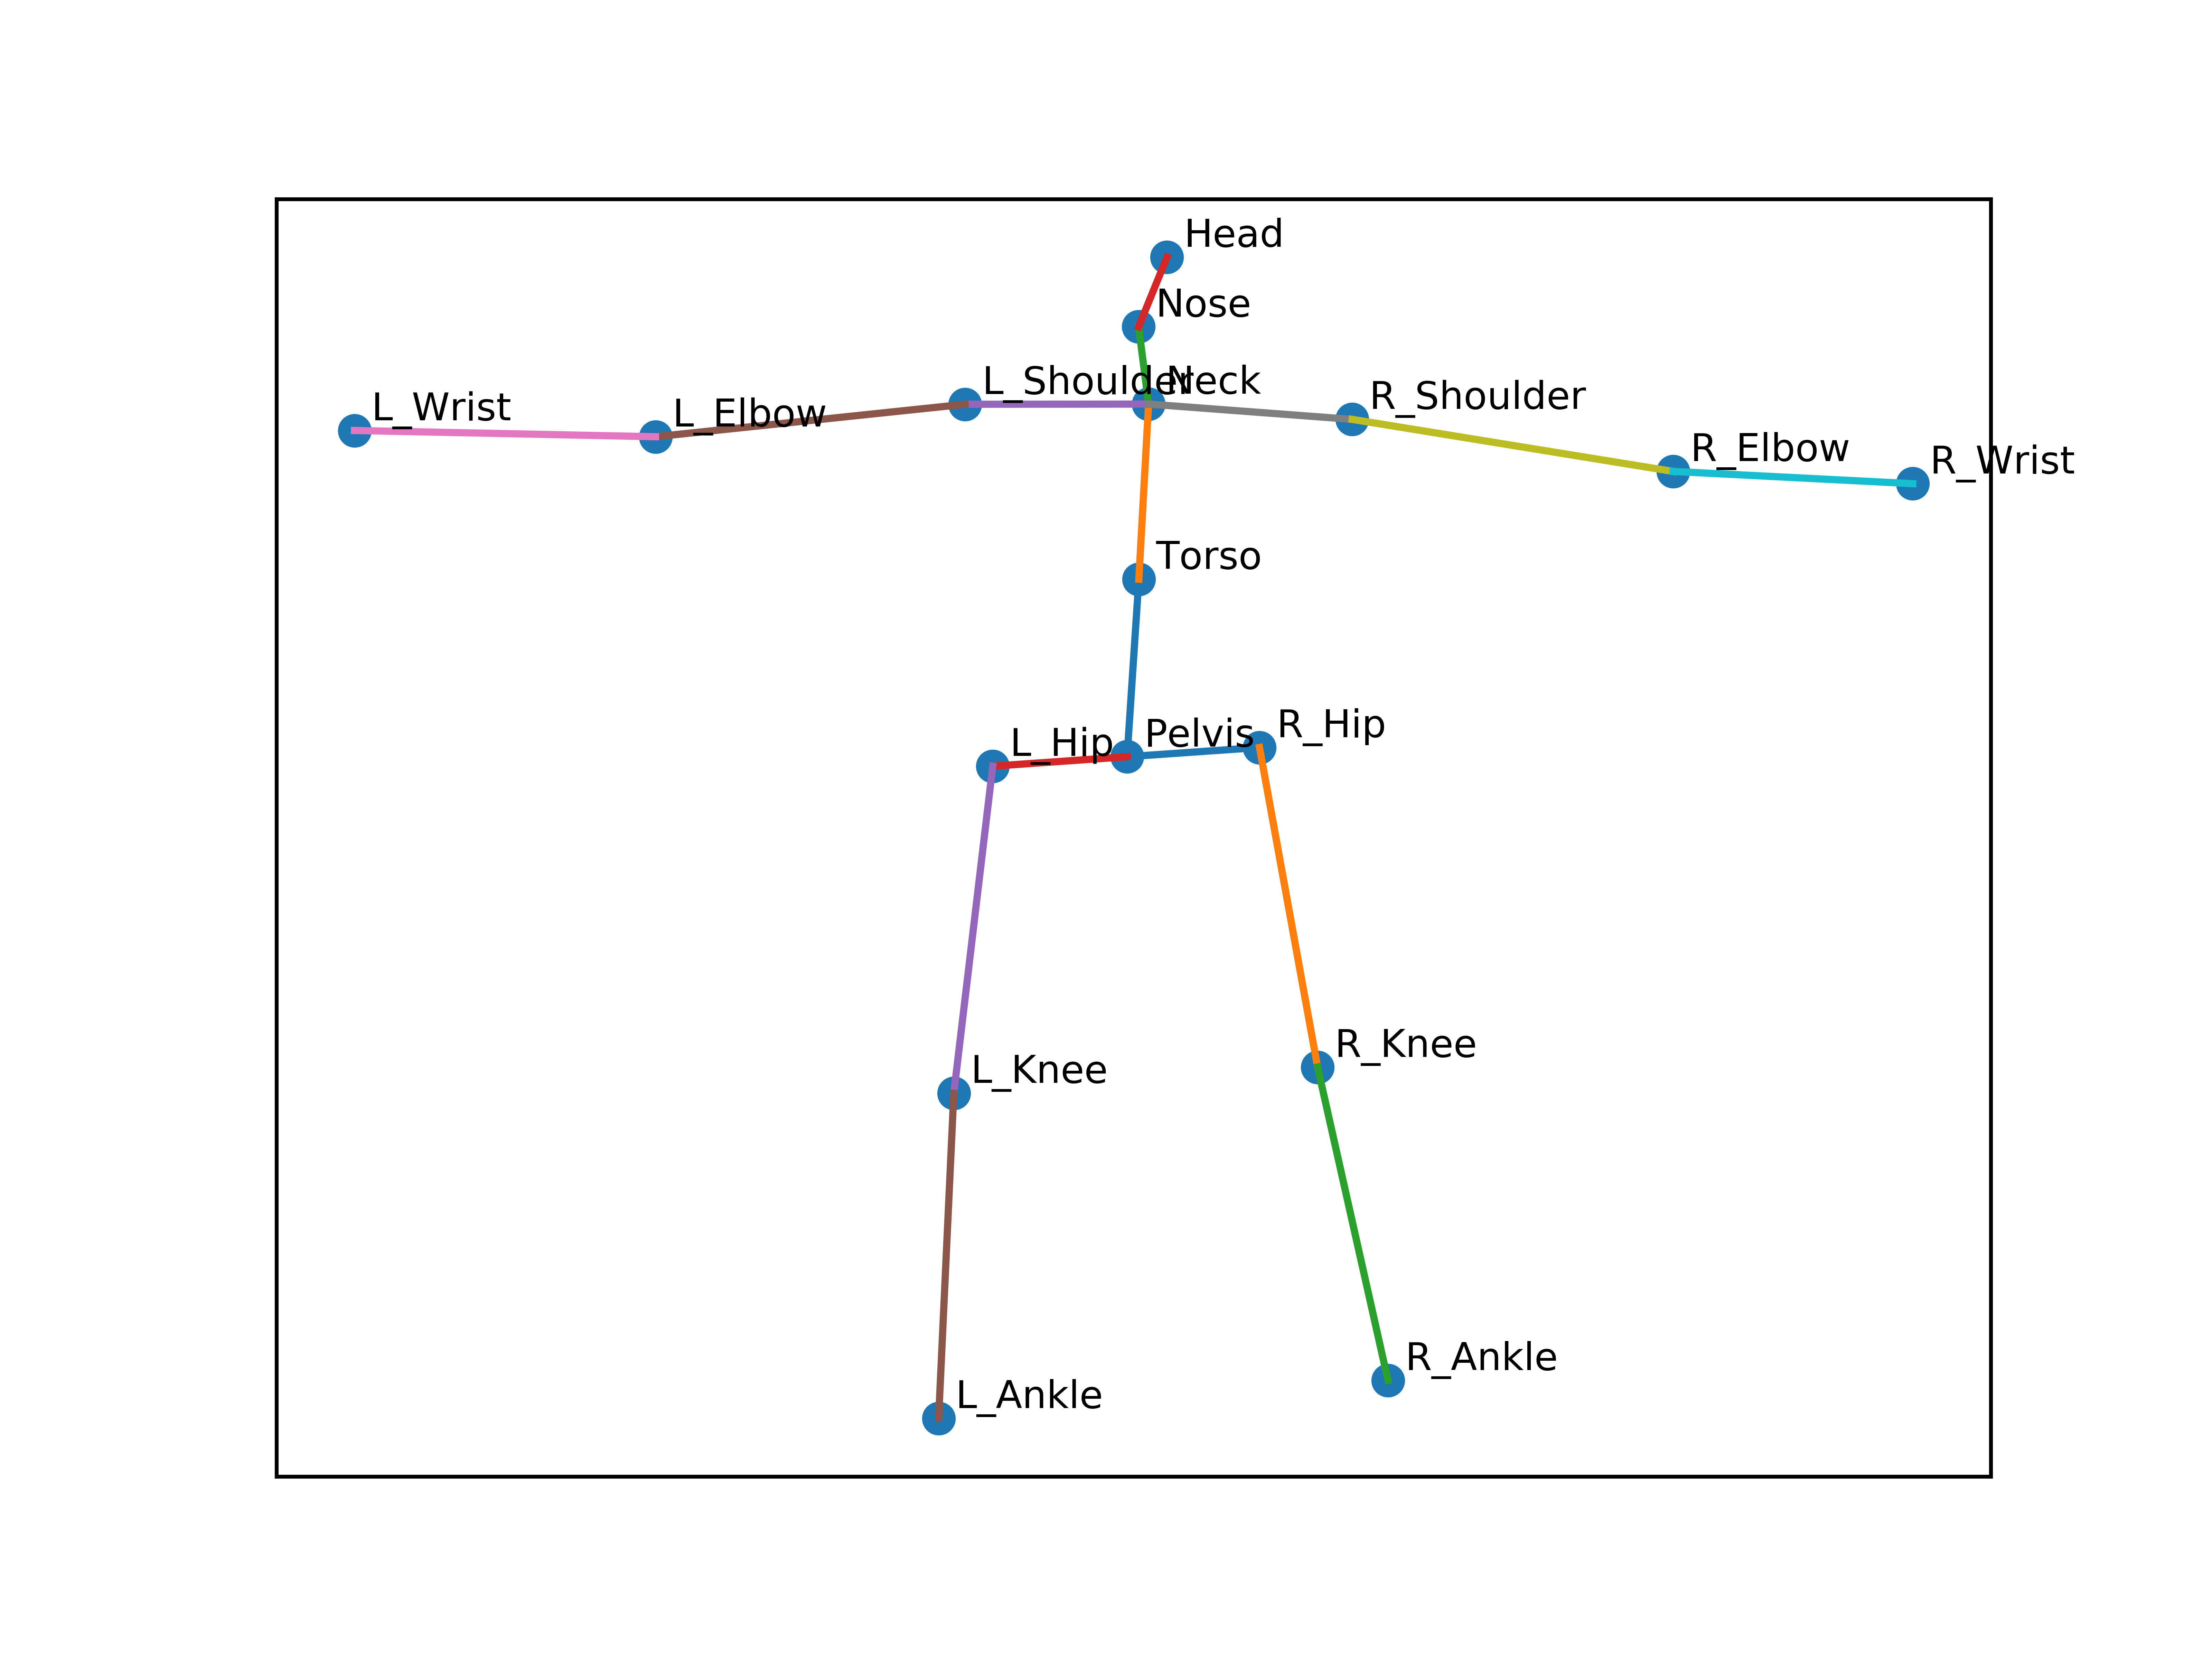
\includegraphics[width=\textwidth]{figures/h36_viz/h362d.png}
        \caption{}
    \end{subfigure}
    \hfill
    \begin{subfigure}[b]{0.3\textwidth}
        \centering
        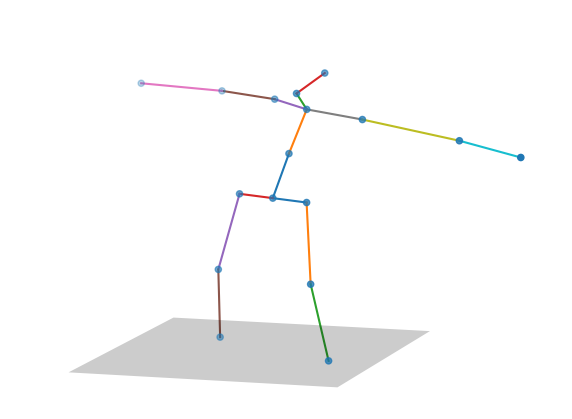
\includegraphics[width=\textwidth]{figures/h36_viz/h363d.png}
        \caption{}
    \end{subfigure}

    \caption{(a) RGB image from one of the 4 cameras. (b) Corresponding 2D pose obtained from the 3D pose to the right with joint labels. (c) Corresponding 3D pose, rotated for a better view of the spatial distribution of the joints}

    \label{fig:h36_sample}
\end{figure}

As illustrated in Fig \ref{fig:h36_data_collection}, the data is collected from a indoor environment with multiple cameras and \ac{mocap} sensors. The obtained coordinates of the 3D pose from \ac{mocap} data are global and is relative to a fixed origin the recording room. In addition to the global 3D pose, camera relative, i.e local 3D pose is also obtained using the camera's location with respect to the global origin. The global poses are useful for methods that try to exploit the multiview information and local poses that are relative to the camera can be used for absolute pose estimation. The 2D pose from each view is obtained by projection the 3D pose using the parameters of the respective camera. This 2D pose is relative to that particular camera and is with respect to the full-scale image that captures the entire scene in the camera's field of view. Along with the RGB images, global and local 3D pose and 2D pose, other metadata is available. This metadata includes intrinsic and extrinsic parameters of each camera, an identifier for each of the samples of a particular action sequence, bounding box coordinates of the human in the full-scale image, subject, action, subaction and camera ids for each sample. This data is processed to suit the task requirements. These details are later presented in section \ref{sec:processing}.

\begin{figure}[h]
    \centering
    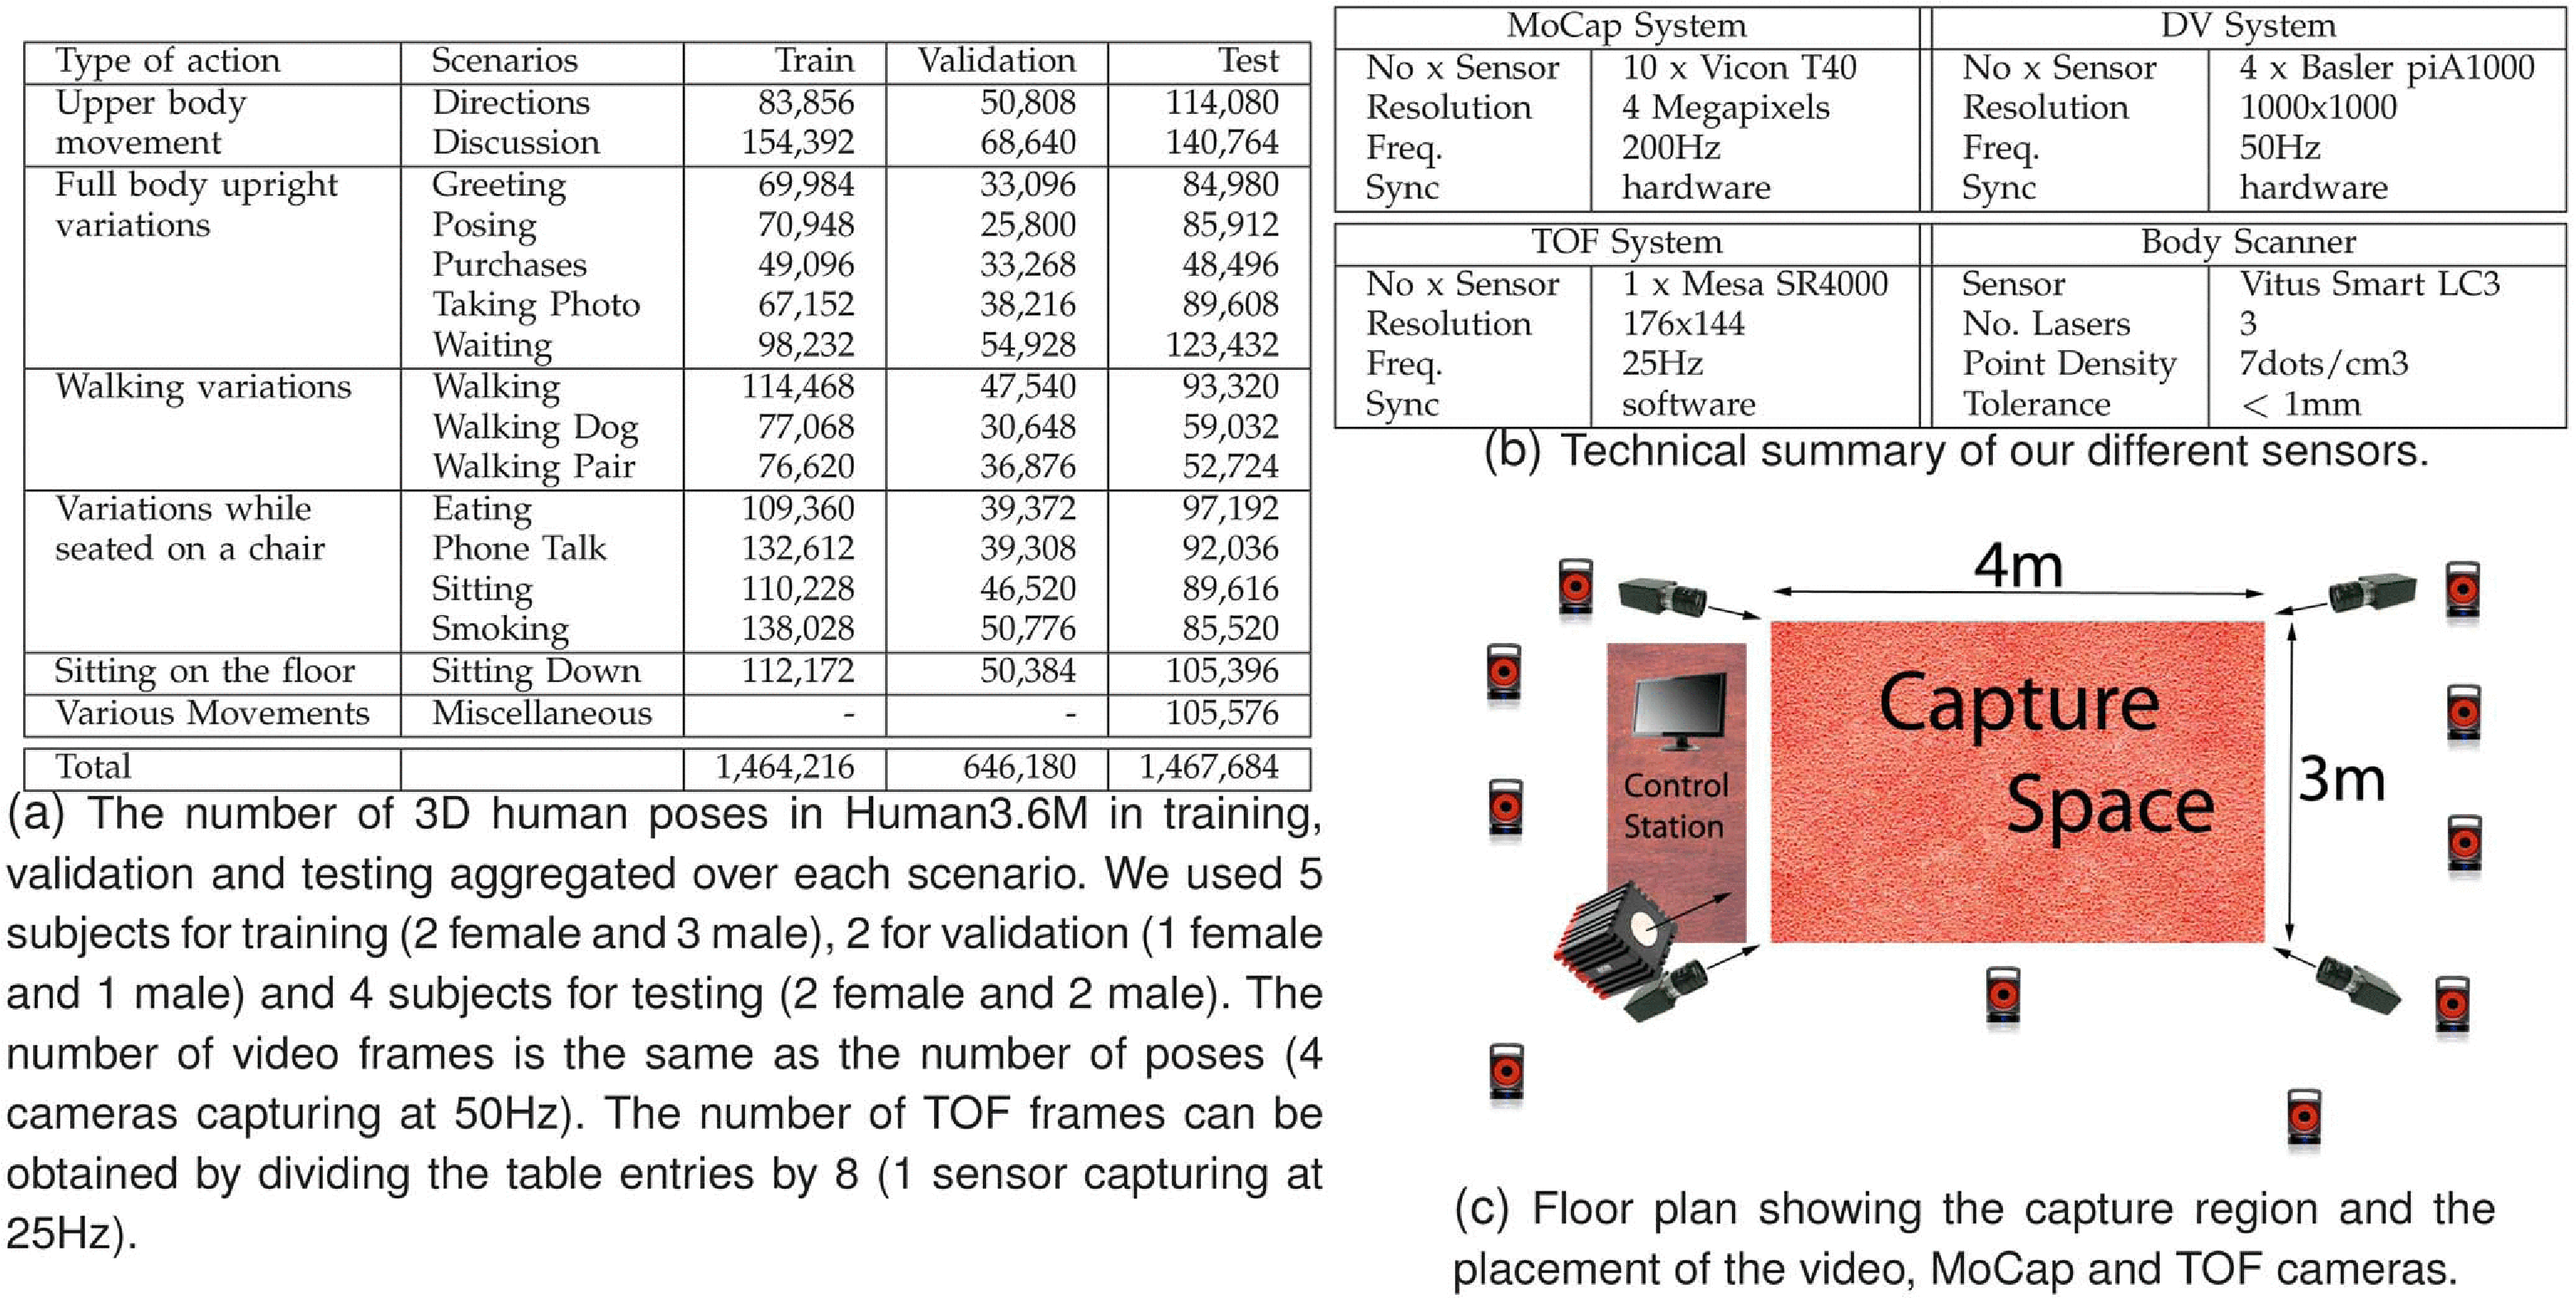
\includegraphics[width=\textwidth]{figures/h36/data_collection.pdf}
    \caption{Human3.6M data collection details. Image source \cite{H3.6}}
    \label{fig:h36_data_collection}
\end{figure}

\section{Camera projection}
\label{camera_projection}

The projection of the poses in the thesis is using a simple pinhole camera model as illustrated in Fig \ref{fig:pinhole}. The image of an object, here a person depicted as 3D pose, is formed on the other side of the camera, or the lens at a distance of $f$. Where $f$ is the focal length of the camera. This image that is formed on the true image plane behind the camera is upside down. For better understanding and comparision the image plane as been translated before the camera and since its before the pinhole, it is not inverted. Assume the two lines passing though from the head and root joints of both the 3D pose and 2D image to the camera make an angle of $\theta$. Also assume the distance between the 3D pose and the camera as $c$, and the height of the pose i.e, distance between the head and the root joint as $k$. Considering the similar traingles formed by the two rays and the line joining the head and root of pose in image and world frame, the ratio of heights to their distance from the camera should be the same. Hence the height of the 2D pose is $k f/c$. This relationship is used in the following sections on data preprocessing. The ground truth 2D as explained earlier is obtained by similar projects taking the camera intrinsic and extrinsic parameters into account.

\begin{figure}[h]
    \centering
    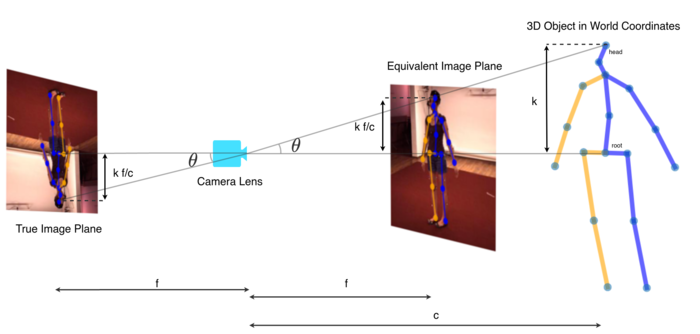
\includegraphics[scale=0.2]{figures/background/pinhole.png}
    \caption{Illustration of a pinhole camera model}
    \label{fig:pinhole}
\end{figure}

\section{Depth Ambiguity and Camera Modeling}
\label{depth_ambiguity_camera_modeling}
One of the main problems discussed in \ref{sec:Related Work} is the depth ambiguity. The Fig \ref{fig:depth_ambiguity_case1} illustrates a case where a 3D pose gives the same 2D pose when scaled and shifted by the same factor, here 2. The second case shows the same 3D pose giving different projections for different focal length i.e the poses are kept the same while scaling the focal length and distance. Hence it is not possible to predict absolute pose from a single view alone. However, works suchs as \cite{CameraDistanceAware} try to tackle these challenges by learning the scale of human based on the features extracted from images. While works such as \cite{repnet,weaklymultiple} that do not use image features learn the camera parameters that are used to project 3D to 2D for learing 3D pose in a self-supervised manner. 

\begin{figure}[h]
    \centering
    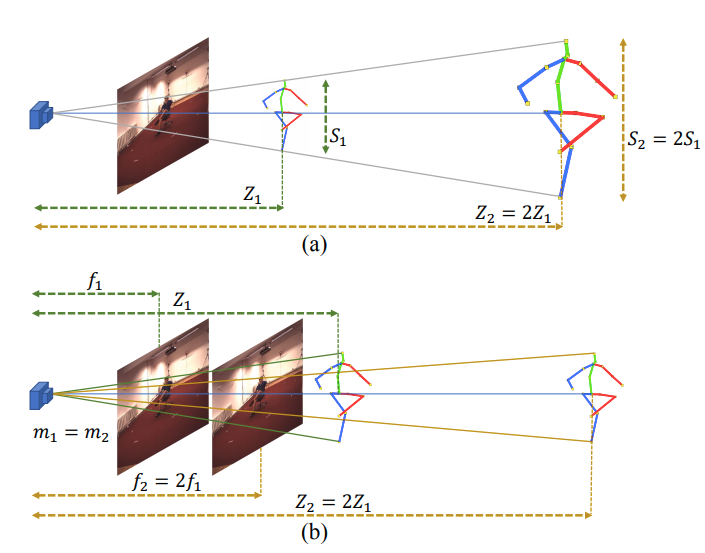
\includegraphics[width=\textwidth]{figures/background/depthambi.png}
    \caption{Cases of depth ambiguity for a given 3D pose (a) Multiple 3D poses that result in the same projection for a camera of a given focal length. (b) Same pose at different distances giving the same projection for different focal lengths.
    Image Source \cite{poselifter}}

    \label{fig:depth_ambiguity_case1}
\end{figure}

Assuming the focal length and distance are known constants, there still exists infinite 3D poses, that give the same 2D projection. However only a smaller subset of poses are plausible i.e pose that can be articulate by the human body. Fig \ref{fig:depth_ambiguity_case2} illustrates a few 3D poses that when projection from the same camera viewpoint produce the same 2D pose (the first image). The first 3D pose (in red and blue) is the ground truth pose used to obtain the 2D pose where the rest of the 3D poses (in mono-colors) are plausible solutions that can be articulated by the human body. 

\begin{figure}[h]
    \centering
    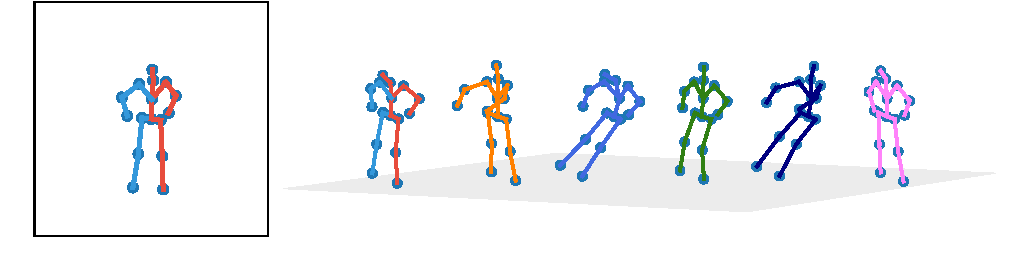
\includegraphics[width=\textwidth]{figures/h36_viz/multiple3d_per_2d.pdf}
    \caption{Cases of depth ambiguity for a given camera and fixed distance from 3D pose. Multiple 3D poses that result in the same projection for a given focal length and placed at the same distance from camera. The variation is only in the depth $z$ component of each joint. Modification of an image from \cite{poselifter}}

    \label{fig:depth_ambiguity_case2}
\end{figure}


\section{Processing}
\label{processing}
The methods explored as part of this thesis, use images, 2D, and 3D human pose from the dataset besides metadata. Where 2D poses are used as training data, 3D poses are only used for evaluation and images are for qualitative analysis. The following describes the modifications done to the raw data for the tasks related to single person detection that are consistantly followed in the field. This is followed by the pre-processing steps done to the data that is specific to the presented work.

As discussed in section \ref{sec:h36m}, the 3D pose in the dataset that is obtained from the marker-based \ac{mocap} is in a global reference frame. These poses using the camera parameters are transformed into the camera coordinate frame. For the task of predicting 3D pose from either images or 2D pose, it is unrealistic to directly estimate all the joints of the pose in a global frame. The works that predict absolute 3D pose are presented in Chapter \ref{chap:background} and are fully supervised or exploit multi-view data and is not in the scope of this thesis. Since the focus is on unsupervised estimation and considering the depth ambiguity challenges we confine the scope to estimating pose relative to an origin point. The pelvis joint is generally considered as the origin or the root joint relative to which the coordinates of other joints are described. 

The full-scale images for such tasks are cropped using the bounding box annotations as a guide to obtain images of aspect ratio 1:1. These cropped images are then scaled to 256x256 images. It important to note that the 2D annotations are relative to the full-scale image and hence the projections are no more synchronized to the images. The translation to these 2D pose are later done exclusively for visualizing the data. Since the image data is not utilized in the training or testing procedures, it is not required to maintain consistency with 2D or 3D annotations. 

The 2D and 3D poses are translated such that the root joint, pelvis is at the origin. Since the pelvis is fixed at the origin, we remove it from the pose after translation so that the network is not required to learn a constant. Removing Pelvis, 16 out of the 17 joints or keypoints remain. The poses are generally normalized before feeding them to the neural network. These are the steps were performed and were sufficient for the initial supervised version of the method. Further steps which are inspired from \cite{amazon1}, are performed to make unsupervised adversarial training possible. 

Considering the different cases of depth ambiguity explained in the previous section, a simple unit pinhole camera is assumed for all the data. That is a camera with a unit focal length, whose image plane is at a distance of 1 unit. Hence the 3D pose that forms an image on this image plane is further from the camera as depicted in the pinhole camera model figure \ref{fig:pinhole}. So the estimated 3D poses can not be at the origin, hence they are fixed at a distance $c$ units. $c$ is set to 10 for all the experiments. It is worth clarifying that only 2D poses are present and 3D are predicted by the neural network. Hence the 2D poses should be processed to achieve this. 

Referring to the pinhole camera figure again \ref{fig:pinhole}, $f$ and $c$ are constants of value 1, 10 respectively. Hence the scale of 3D pose that should be ideally predicted by the model is 10 times that of the 2D pose. The predicted 3D is projected to 2D just by dividing the $x$, $y$ coordinates by the $z$ component as it is a simple pinhole camera. The pose is rotated and project again and passed to a discriminator network following the \ac{vae}-\ac{gan} network explained in Preliminary Concepts section \ref{sec:Preliminary}. For numerical stability we process the 2D pose such that the height of the desired 3D pose is of approximately of unit length. To achieve this the 2D poses are scaled such that the mean distance from the head to the root joint is 1/10 ($k f/c$). 

Following the above processing procedure, the predicted 3D pose is not to scale with the ground truth 3D poses. Following the related unsupervised works sucha s \cite{amazon1}, we evaluate the 3D pose by aligning the prediction to the ground truth pose using rigid body alignment also referred to as Procrustes alignement as illustrated in Fig \ref{fig:procrustes}. Since the transformation is taken care by the algorithm, no other post-processing procedure is required for the proposed unsupervised method. More details about the evaluation is preseneted in chapter \ref{chap:method}, the Method.


%FIXME \section{Procrustes Alignment} or even a cite a resource

\begin{figure}
    \centering
    \begin{subfigure}[b]{0.25\textwidth}
        \centering
        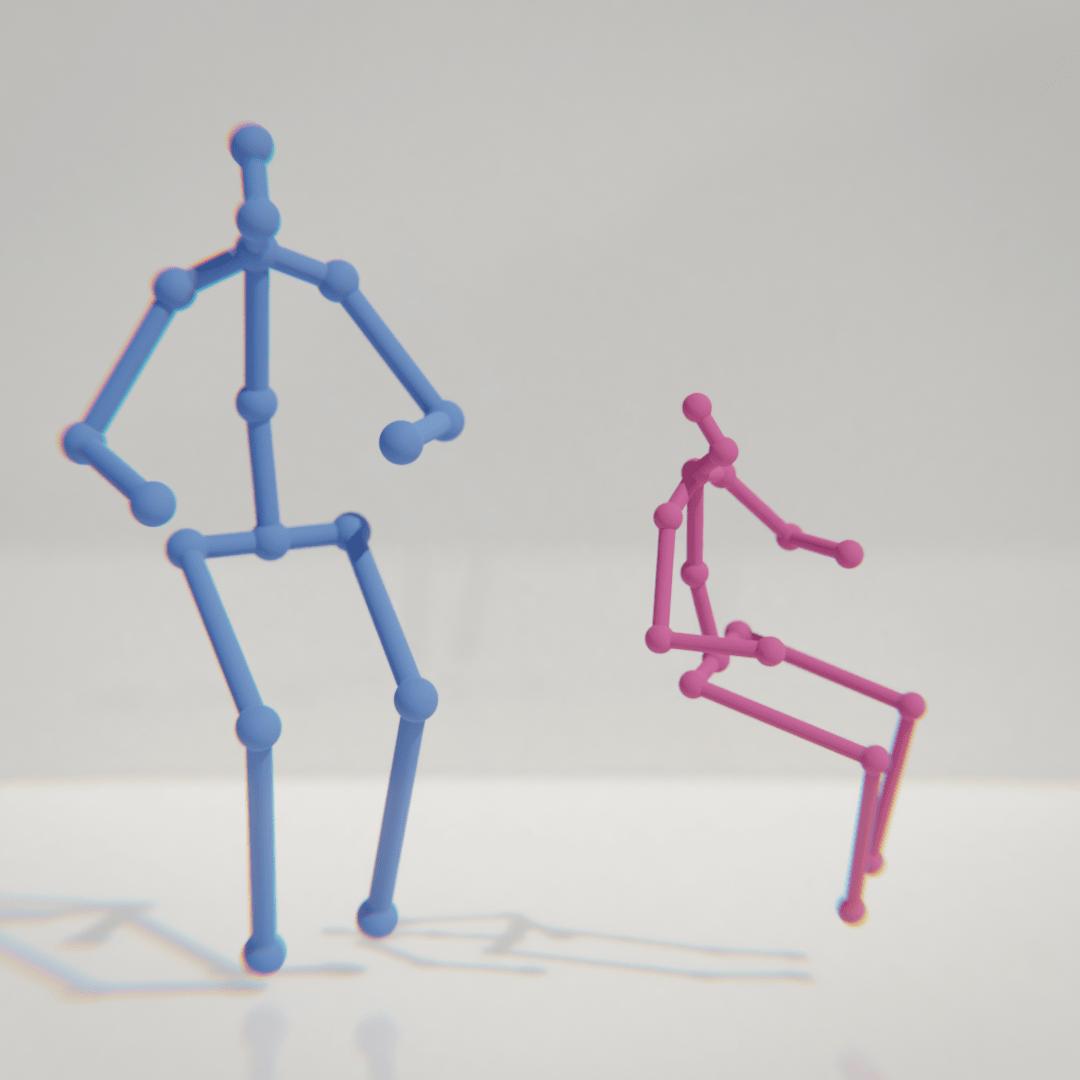
\includegraphics[width=\textwidth]{figures/h36_viz/proc_raw.png}
        \caption{Prediction and Ground Truth}
    \end{subfigure}
    \hfill
    \begin{subfigure}[b]{0.25\textwidth}
        \centering
        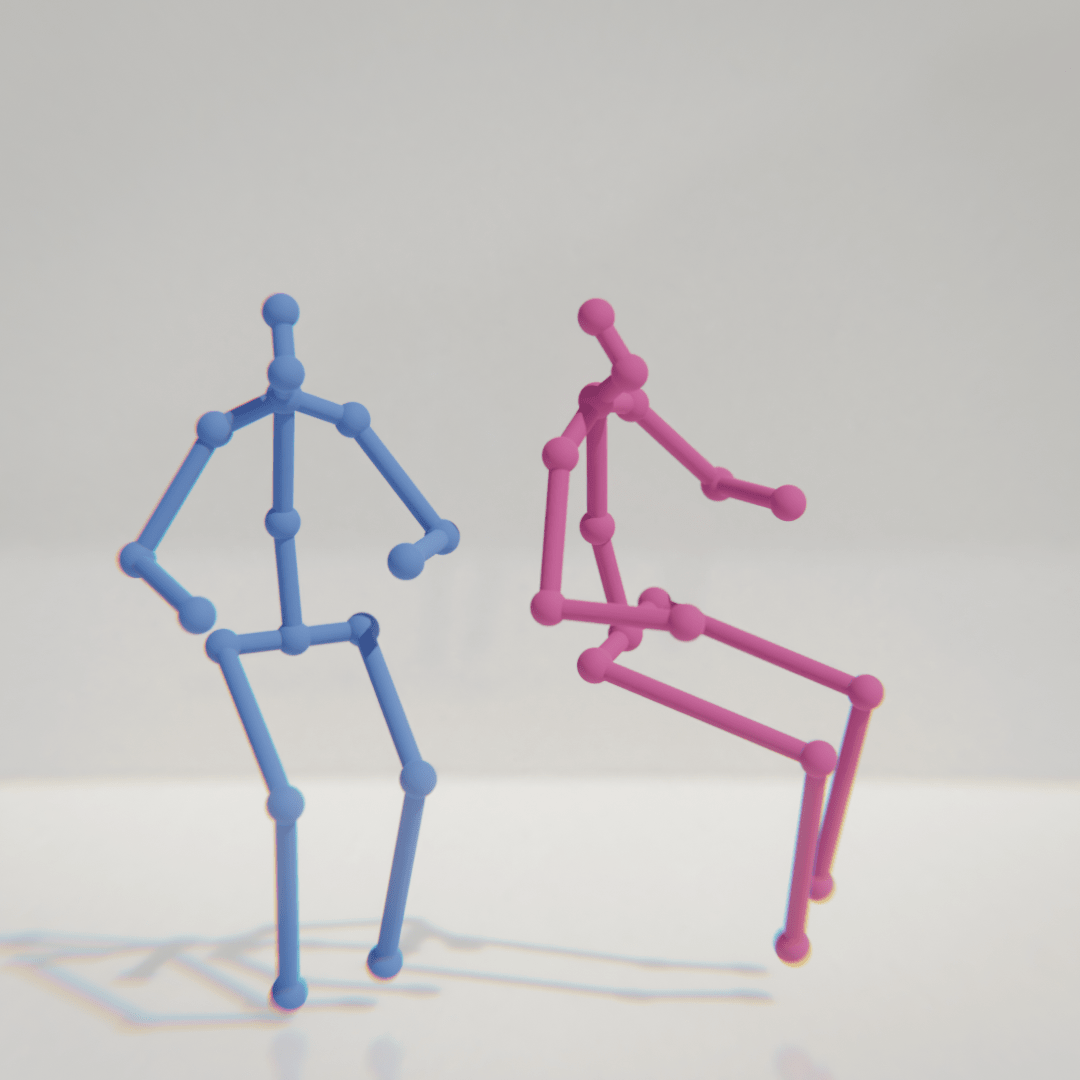
\includegraphics[width=\textwidth]{figures/h36_viz/proc_scale.png}
        \caption{Scale to the same size}
    \end{subfigure}
    \hfill
    \begin{subfigure}[b]{0.25\textwidth}
        \centering
        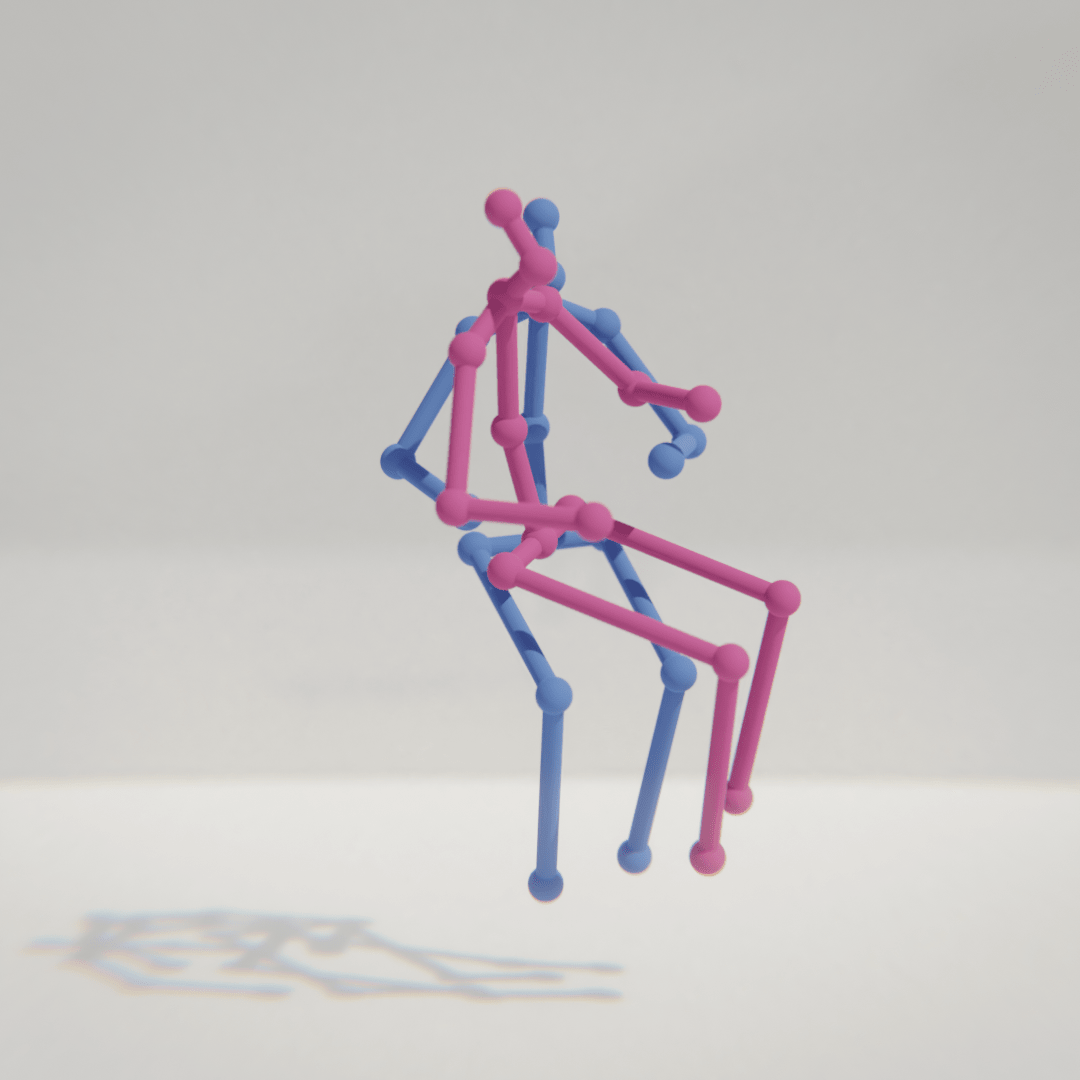
\includegraphics[width=\textwidth]{figures/h36_viz/proc_pos.png}
        \caption{Translated to the same position}
    \end{subfigure}
    \hfill
    \begin{subfigure}[b]{0.25\textwidth}
        \centering
        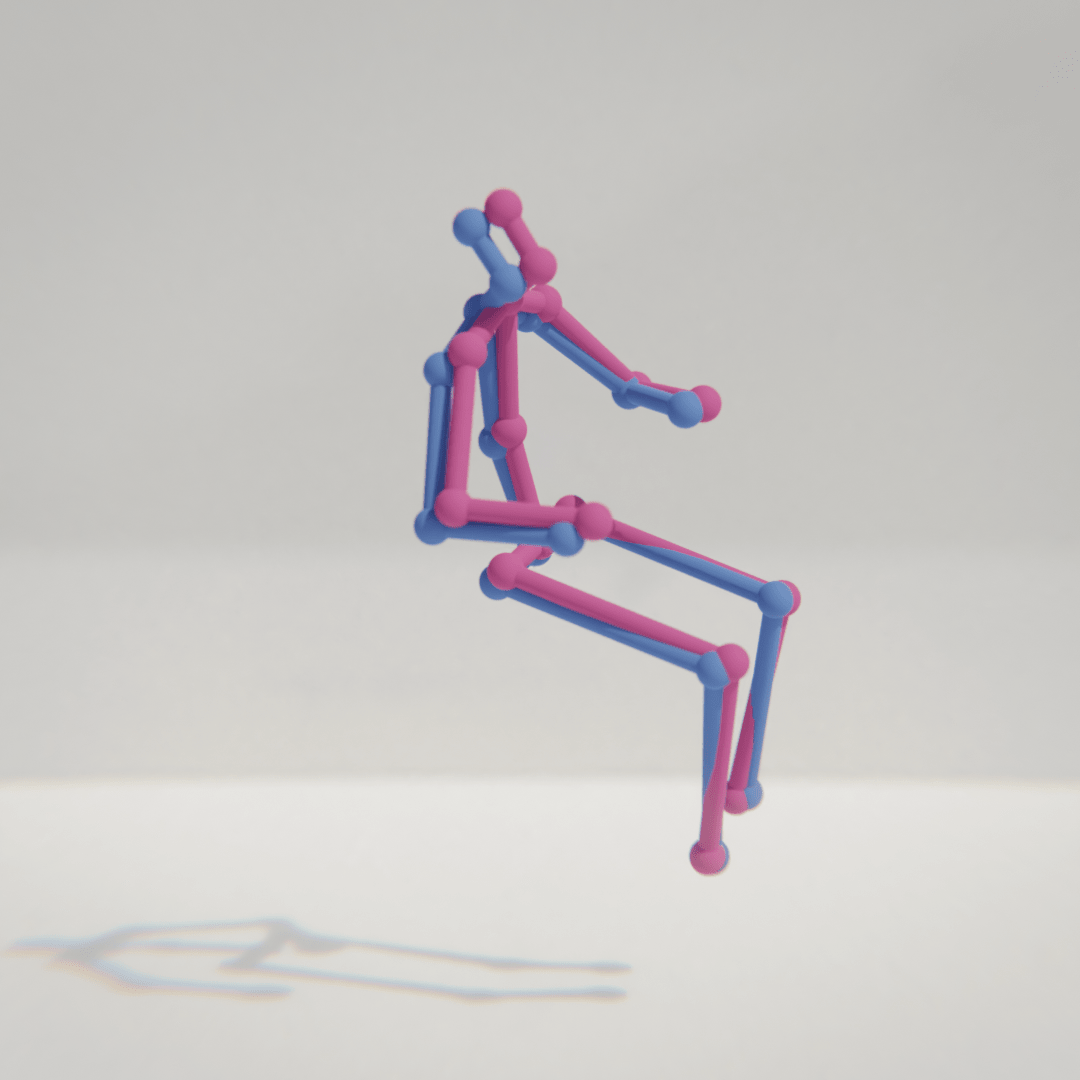
\includegraphics[width=\textwidth]{figures/h36_viz/proc_rot.png}
        \caption{Rotated to the same orientation}
    \end{subfigure}
    \caption{Procrustes alignement of a 3D pose (pose in blue) to minimize the distance to the reference pose (pose in pink)}
    \label{fig:procrustes}
\end{figure}
